
% Preamble
\documentclass[11pt]{report}

% Packages
\usepackage{amsmath}
\usepackage{graphicx}
\usepackage{color}
\usepackage[table,xcdraw]{xcolor}
\usepackage{multirow}


% set image file paths
\graphicspath{ {../../fuzzy/output/mamdani\_bell\_v9/io\_graphs/} }


\title{Funky Systems and Neural Networks}
\author{Jéssica Consciência e Tiago Leite}


\begin{document}
\maketitle
\newpage

\part{Fuzzy System}

%% Texto ainda por melhorar!!
Firstly we started by deciding between which type of fuzzy system
we should implement: Mamdani, Takagi-Sugeno or Tsukamoto. From the
project statement we observe that the output \textit{CLPVariation}
is not any clear function of the input, rulling out Takagi-Sugeno,
also meaning that our output is a \bold{Fuzzy Set}. If we wish for
our output to be monotonic then the choice would be Tsukomoto, since
we did not want this restriction and decided for starting with a simple
approach then later on adding difficulty when needed.
(Early on we decided to try to make data-driven decisions with an iterative
improving process)

\section{First Iterations}
For the first iteration the choice of variables, through common sense, \textit{ProcessorLoad},
 \textit{MemoryUsage} and \textit{Latency} were the first choices, and for output \textit{CLP}\}.
We chose triangular Membership Functions with 4 intervals for each variable (low, medium, high, critical)
for \textit{ProcessorLoad} and \textit{MemoryUsage} and (poor, fair, good, great) for \textit{Latency}.
\\?Show image?\\
Then, we decided to experiment with exchanging the membership function to gaussian
\\ 3D graph of Gaussian \\
Whilst experimenting different membership functions the necessity of visualizing arose,
a helper script was developed [fuzzy/visualization/fuzzy\_system\_to\_dataframe] that
 receives the FuzzySystem python object and dynamically creates a dataframe to aid in
plotting the membership functions.

\section{Generalized Bell}
We decided to experiment with a more generic Membership function, so we
extended simpful's Base Membership Function class and created Bell\_MF [in fuzzy/models/bell\_mf.py].
The first results are shown in the figure bellow.

%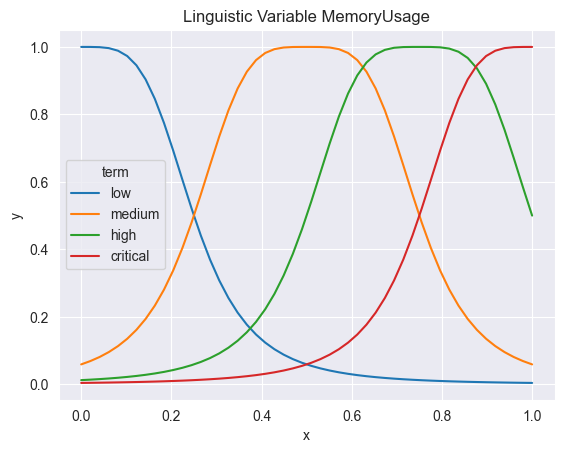
\includegraphics[width=0.5]{../../fuzzy/output/mamdani_bell/io_graphs/MemoryUsage.png}
%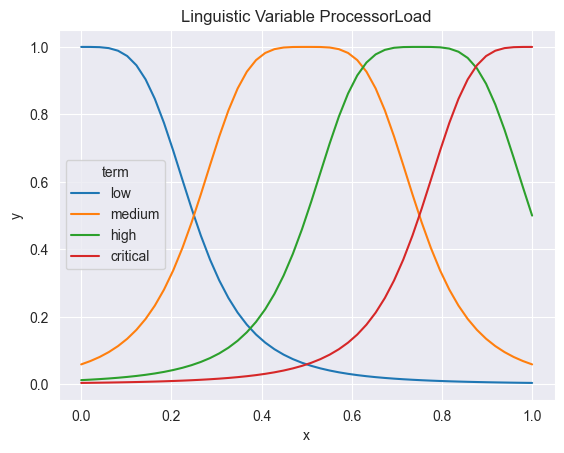
\includegraphics[width=0.5]{../../fuzzy/output/mamdani_bell/io_graphs/ProcessorLoad.png}
%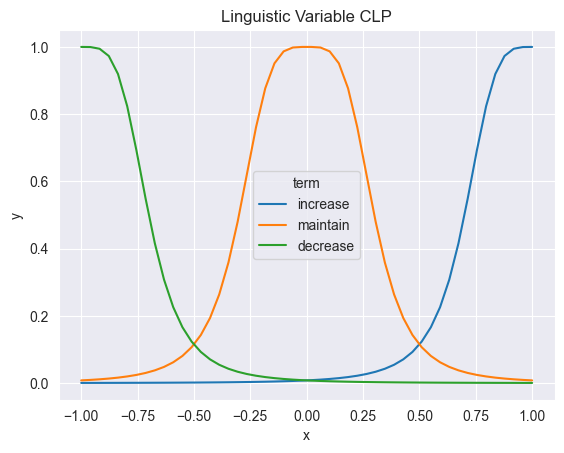
\includegraphics[width=0.5]{../../fuzzy/output/mamdani_bell/io_graphs/CLP.png}

%%
\section{Architecture}
This should contain choice of architecture and why.

\section{Membership Functions}
all the membership functions and linguistic terms

\begin{figure}

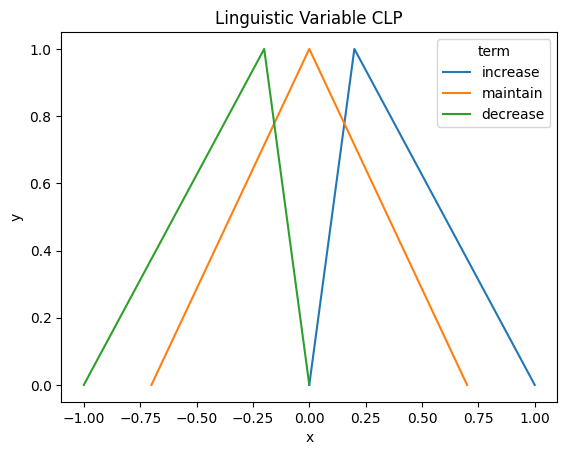
\includegraphics{CLP.png}
%\begin{tabular}[ccc]
%    \subfloat[caption]{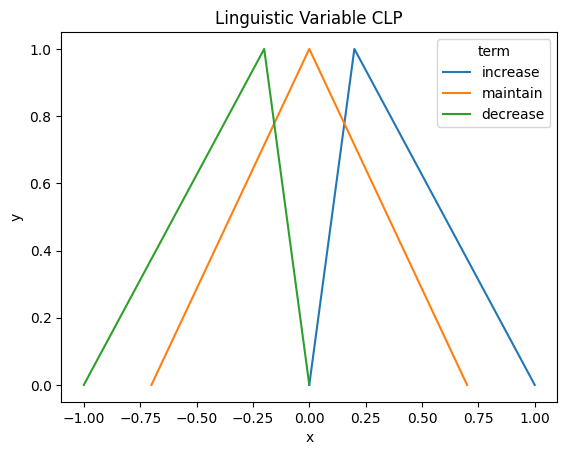
\includegraphics[width=.3\textwidth]{CLP.png}} & % noqa
%    \subfloat[caption]{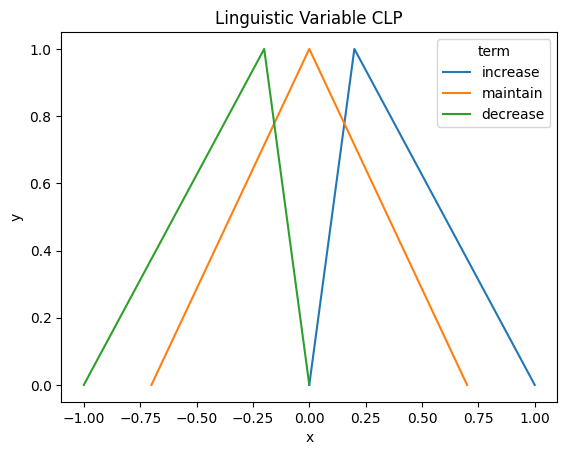
\includegraphics[width=.3\textwidth]{CLP.png}} &
%    \subfloat[caption]{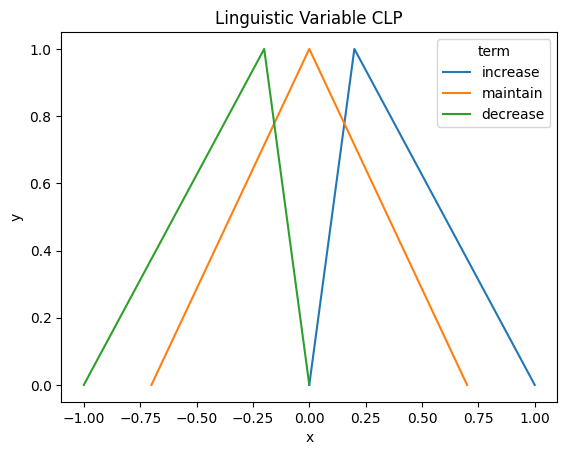
\includegraphics[width=.3\textwidth]{CLP.png}} \\
%\end{tabular}
\end{figure}

\section{Rules}
rules

\begin{table}[]
\begin{tabular}{|
>{\columncolor[HTML]{9698ED}}c l|cccc|}
\hline
\multicolumn{2}{|c|}{\cellcolor[HTML]{FFCC67}{\color[HTML]{333333} }}                                & \multicolumn{4}{c|}{\cellcolor[HTML]{9698ED}Latency}                                                        \\ \cline{3-6}
\multicolumn{2}{|c|}{\multirow{-2}{*}{\cellcolor[HTML]{FFCC67}{\color[HTML]{333333} CLP Variation}}} & \multicolumn{1}{l|}{low} & \multicolumn{1}{l|}{moderate} & \multicolumn{1}{l|}{high} & \multicolumn{1}{l|}{very high} \\ \hline
\multicolumn{1}{|c|}{\cellcolor[HTML]{9698ED}}                                     & low             & \multicolumn{1}{c|}{IS}  & \multicolumn{1}{c|}{IS}       & \multicolumn{1}{c|}{I}    & I                              \\ \cline{2-6}
\multicolumn{1}{|c|}{\cellcolor[HTML]{9698ED}}                                     & moderate        & \multicolumn{1}{c|}{I}   & \multicolumn{1}{c|}{I}        & \multicolumn{1}{c|}{I}    & I                              \\ \cline{2-6}
\multicolumn{1}{|c|}{\cellcolor[HTML]{9698ED}}                                     & high            & \multicolumn{1}{c|}{M}   & \multicolumn{1}{c|}{M}        & \multicolumn{1}{c|}{D}    & D                              \\ \cline{2-6}
\multicolumn{1}{|c|}{\multirow{-4}{*}{\cellcolor[HTML]{9698ED}System Load}}        & critical        & \multicolumn{1}{c|}{DS}  & \multicolumn{1}{c|}{DS}       & \multicolumn{1}{c|}{DS}   & DS                             \\ \hline
\end{tabular}
\end{table}


\section{Results}


\part{Neural Networks}



\end{document}
